\documentclass{beamer}
\usepackage{graphicx} % Required for inserting images

\usepackage[utf8]{inputenc}
\usepackage[T1]{fontenc}
\usepackage{lmodern}
\usepackage{amsmath,amssymb}
\usepackage{microtype}
\usepackage{ellipsis}
%\usepackage[ngerman]{babel}
\let\openbox\undefined
\usepackage{mathtools}
% \usepackage{enumitem}
\let\openbox\undefined
\usepackage{amsthm}
\usepackage{thmtools}
\usepackage{graphicx}
\usepackage{stmaryrd}
\usepackage{tikz}
\usetikzlibrary{positioning}
\usepackage{algpseudocode}
\usepackage[absolute,overlay]{textpos}
\usepackage{url}
\usepackage[
backend=biber,
style=numeric,
]{biblatex}
\addbibresource{references.bib}
\usepackage[normalem]{ulem}
\usepackage{verbatim}
\usepackage{subcaption} % allow for subfigures

\usepackage[ruled, algosection]{algorithm2e}


\declaretheoremstyle[
  spaceabove=\parsep,
  spacebelow=0,
  headfont=\bfseries,
  notefont=\bfseries,
  notebraces={(}{)},
  bodyfont=\normalfont,
  postheadspace=.5em
]{definition}

\newtheoremstyle{plain}         % name
    {\parsep}                   % Space above
    {}                          % Space below
    {\itshape}                  % Body font
    {}                          % Indent amount
    {\bfseries}                 % Theorem head font
    {.}                         % Punctuation after theorem head
    {.5em}                      % Space after theorem head
    {\thmname{#1}\thmnumber{ #2}\thmnote{ \bfseries (#3)}}                 % Theorem head spec (can be left empty, meaning ‘normal’)

\theoremstyle{plain}

% \declaretheorem[sharenumber=algocf]{theorem}
% \declaretheorem[sharenumber=algocf]{lemma}
% \declaretheorem[sharenumber=algocf]{corollary}
\declaretheorem[sharenumber=algocf]{proposition}

% \declaretheorem[sharenumber=algocf]{definition}
% \declaretheorem[sharenumber=algocf]{example}
\declaretheorem[sharenumber=algocf]{remark}
\declaretheorem[sharenumber=algocf]{notation}

\renewcommand\qedsymbol{$\square$}

\newcommand\R{\mathbb R}
\newcommand\Z{\mathbb Z}
\newcommand\N{\mathbb N}
\newcommand\C{\mathbb C}
\newcommand{\Q}{\mathbb Q}
\newcommand{\F}{\mathbb{F}}
\newcommand{\ass}{\underline{Assume:}  }
\newcommand{\zz}{\underline{t.s.:}  }

\renewcommand{\phi}{\varphi}
\renewcommand{\epsilon}{\varepsilon}


\newcommand{\stab}{\mathrm{Stab}}
\newcommand{\conv}{\mathrm{conv}}
\newcommand{\vol}{\mathrm{vol}}
% \newcommand{\min}{\text{min}}
% \newcommand{\max}{\text{max}}
% \newcommand{\ker}{\text{ker}}
\newcommand{\im}{{\mathrm{im}}}
\newcommand{\GL}{\mathrm{GL}}
\newcommand{\Aut}{{\mathrm{Aut}}}

\newcommand{\T}{\mathcal{T}}
\renewcommand{\P}{\mathcal{P}}
\renewcommand{\L}{\mathcal{L}}

\usetheme[compress]{Berlin}
\setbeamertemplate{footline}[frame number]{}
\setbeamertemplate{navigation symbols}{}
\setbeamertemplate{footline}{}

% Change alert block colors

% 1- Block title (background and text)
\setbeamercolor{block title alerted}{fg=white, bg=orange}

% 2- Block body (background)
\setbeamercolor{block body alerted}{bg=orange!25}

\makeatletter
\beamer@theme@subsectionfalse%
\makeatother


\title{Visualising GAP objects: \\current status and the future}
\author{Lukas Schnelle}
\date{GAPDays Summer 2026}


\begin{document}

% remove dots on first slide
\frame[plain]{\titlepage}

\section{Current status}
\begin{frame}
    TODO: motivation
\end{frame}

\begin{frame}
    Currently there are multiple packages, which provide functionality to visualise GAP objects. First we will give an (possibly incomplete) overview of them with some examples.
\end{frame}

% \section{XGAP}
\begin{frame}{XGAP (By Frank Celler and Max Neunh\"offer)}
    Provides a GUI in which e.g. subgroup lattices can be investigated. Needs to be started separately. \\
    
\includegraphics[width=\textwidth]{images/xgap-0.png}
\end{frame}

\begin{frame}
    \centering
    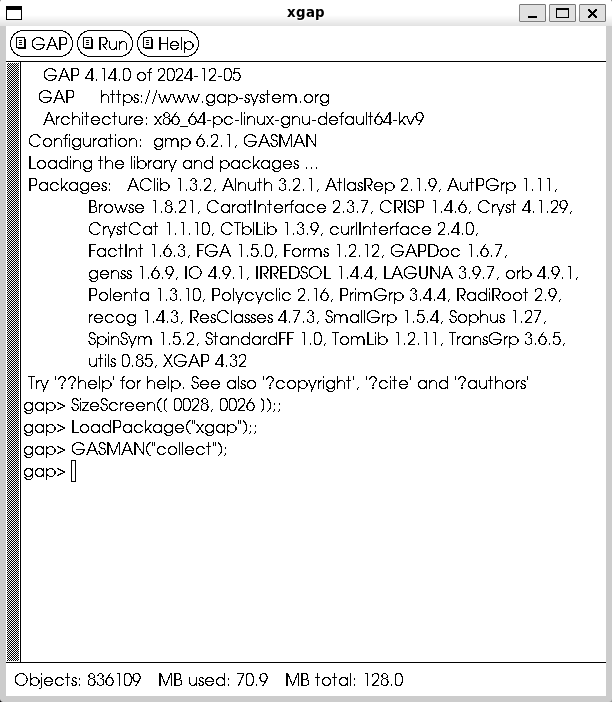
\includegraphics[width=0.7\textwidth]{images/xgap-1.png}
\end{frame}

\begin{frame}
    \centering
    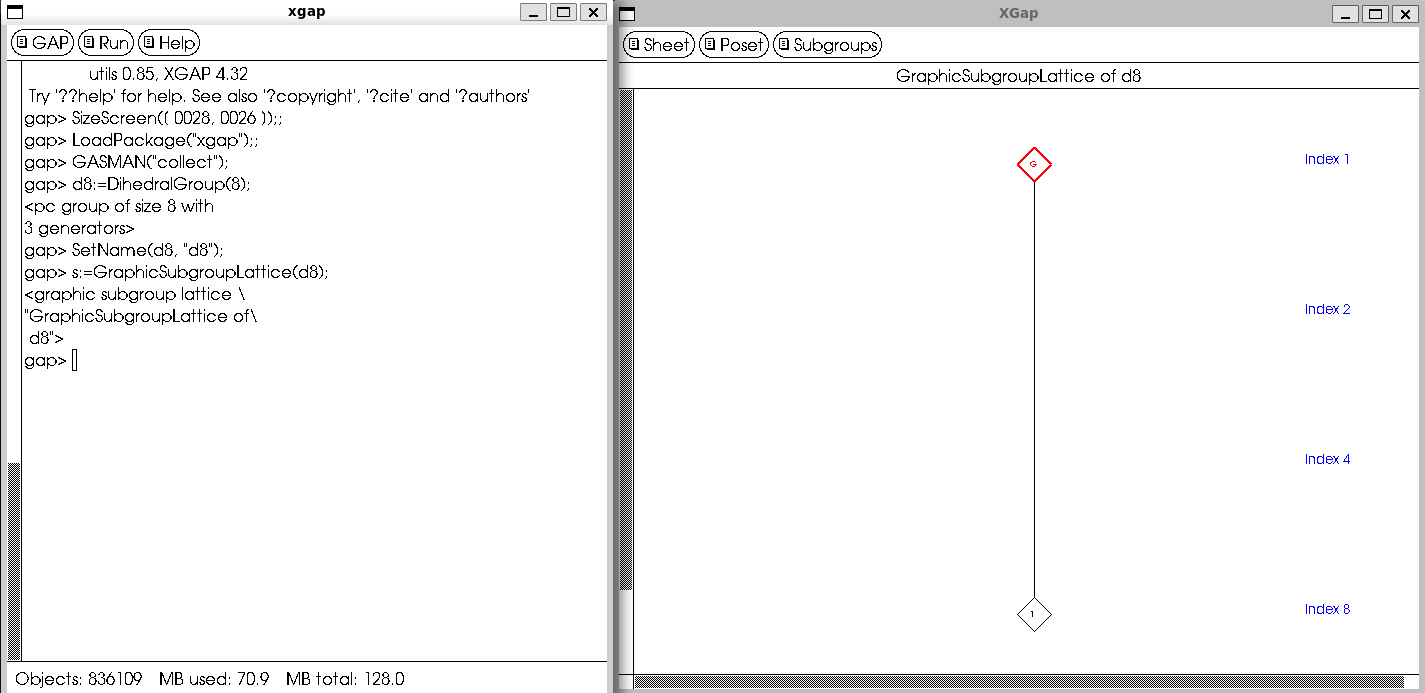
\includegraphics[width=1\textwidth]{images/xgap-2.png}
\end{frame}

\begin{frame}
    \centering
    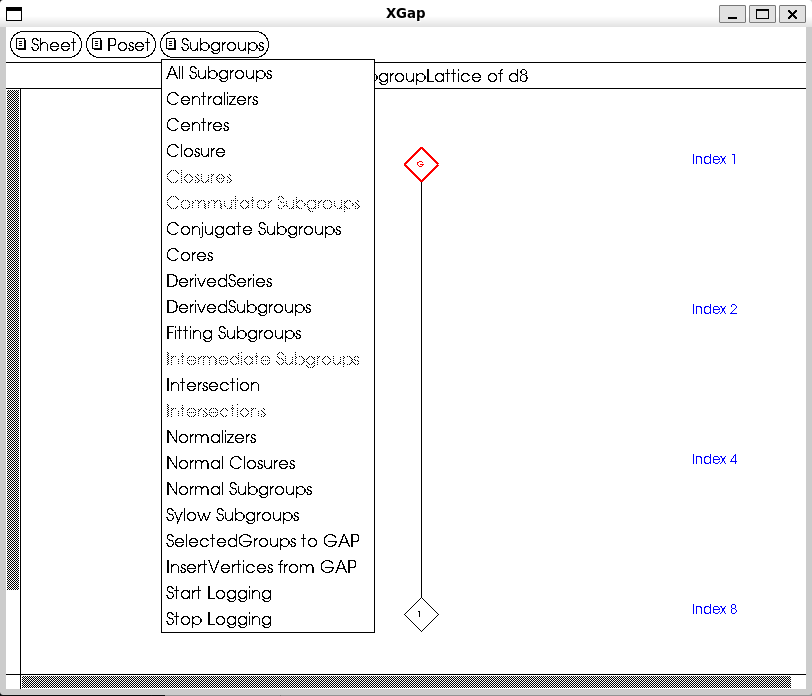
\includegraphics[width=0.9\textwidth]{images/xgap-3.png}
\end{frame}

\begin{frame}
    \centering
    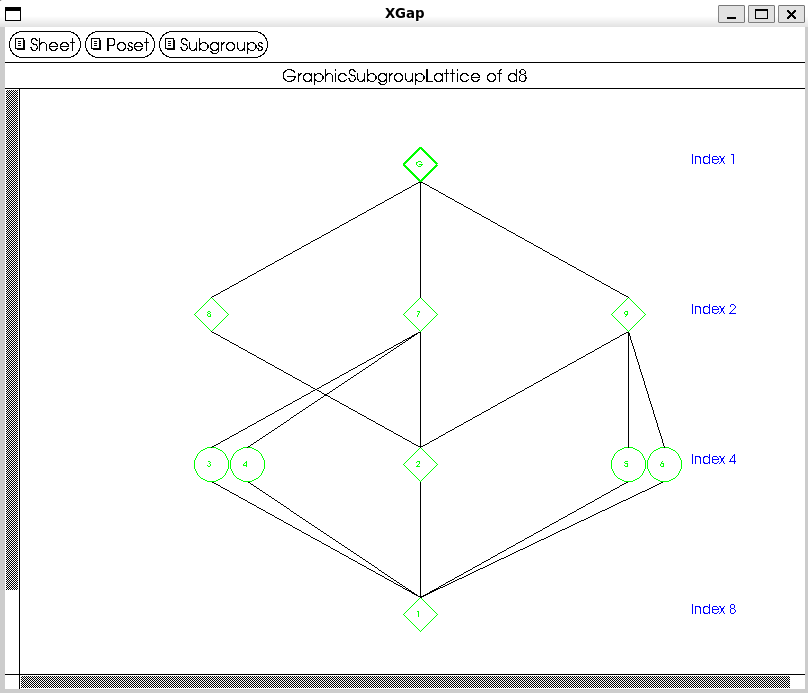
\includegraphics[width=0.9\textwidth]{images/xgap-4.png}
\end{frame}

\begin{frame}
    \begin{exampleblock}{Advantages}
        \begin{itemize}
            \item Direct GUI to use
            \item Freely movable visualisation
        \end{itemize}
    \end{exampleblock}
    \pause
    \begin{alertblock}{Challenges}
        \begin{itemize}
            \item Needs to be started standalone
            \item Needs to be adjusted to every OS
        \end{itemize}
    \end{alertblock}
\end{frame}

% \section{francy}
\begin{frame}{francy (by Manuel Martins)}
    \begin{exampleblock}{Idea}
        Allow the XGAP system to run in a Jupyter Notebook.
    \end{exampleblock}
    \begin{alertblock}{Status}
        I was not able to get this running.
    \end{alertblock}
\end{frame}

\begin{frame}
    \centering
    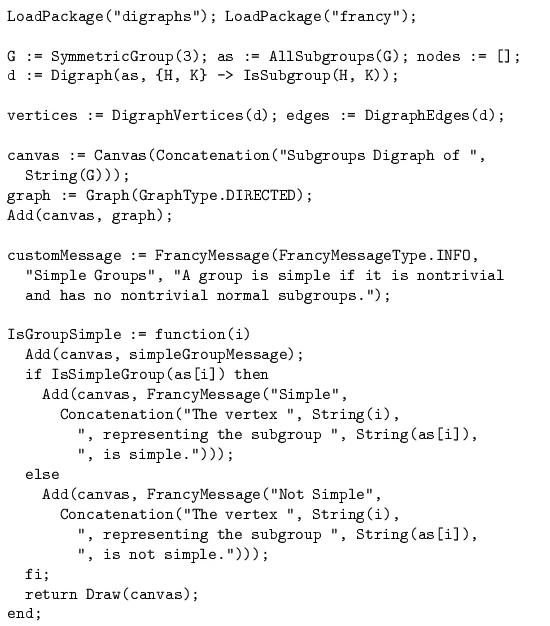
\includegraphics[width=0.7\textwidth]{images/francy-1.png}
\end{frame}

\begin{frame}
    \centering
    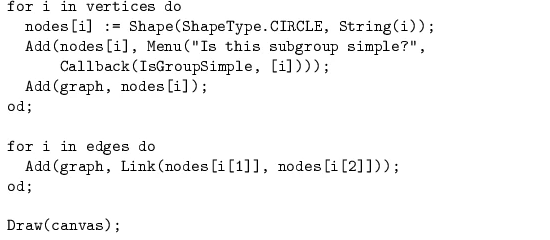
\includegraphics[width=0.7\textwidth]{images/francy-2.png}\\
    (from \cite{francy2018})
\end{frame}

\begin{frame}
    \centering
    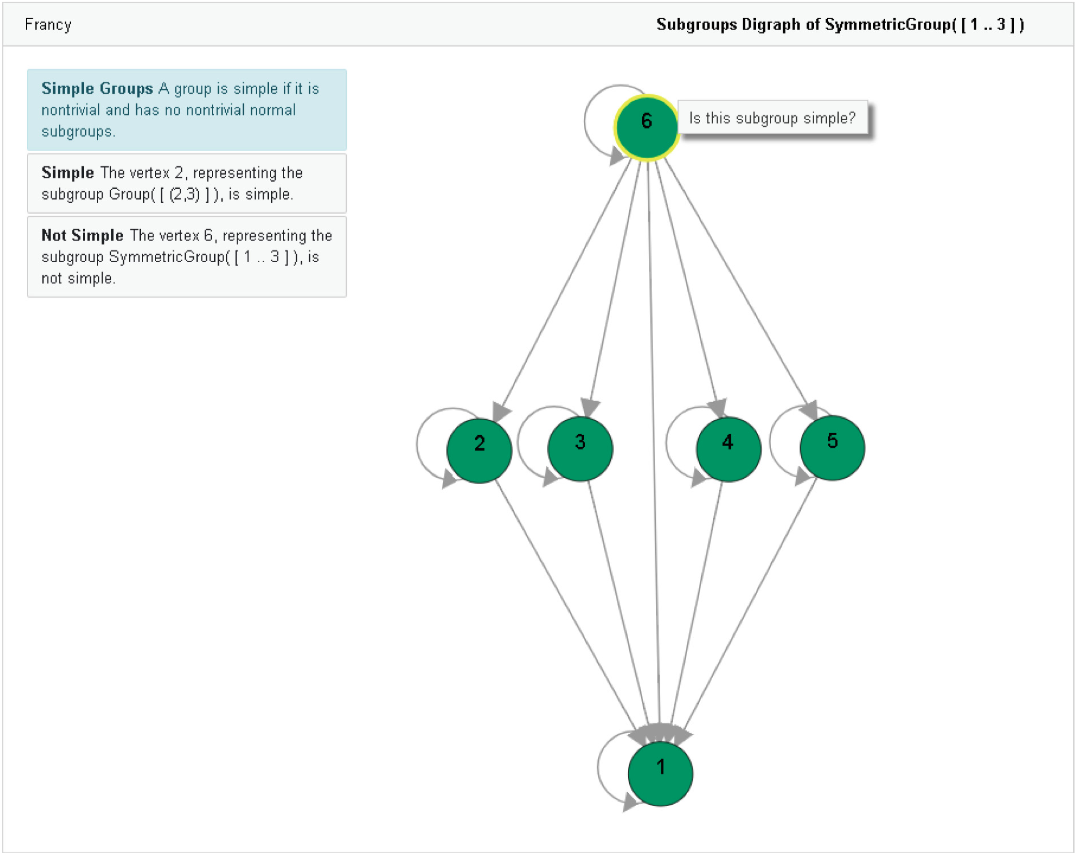
\includegraphics[width=0.9\textwidth]{images/francy-3.png}\\
    (from \cite{francy2018})
\end{frame}

\begin{frame}
    \begin{exampleblock}{Advantages}
        \begin{itemize}
            \item Runs in browser
            \item Highly customisable
        \end{itemize}
    \end{exampleblock}
    \pause
    \begin{alertblock}{Challenges}
        \begin{itemize}
            \item Needs additional installation of Jupyter
        \end{itemize}
    \end{alertblock}
    \pause
    \begin{block}{Other packages}
        \begin{itemize}
            \item jupyterviz
            \item semigroupviz
        \end{itemize}
    \end{block}
\end{frame}

\subsection{SgpViz}
\begin{frame}{SgpViz (by Manuel Delgado and José João Morais)}
    \begin{exampleblock}{Semigroup visualisation}
        \begin{itemize}
            \item Can visualise e.g. Cayley graphs
            \item Using graphviz
        \end{itemize}
    \end{exampleblock}
    \centering
    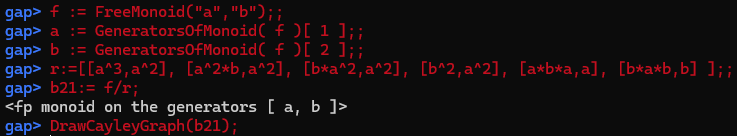
\includegraphics[width=0.9\textwidth]{images/sgpviz-1.png}
\end{frame}

\begin{frame}
    \centering
    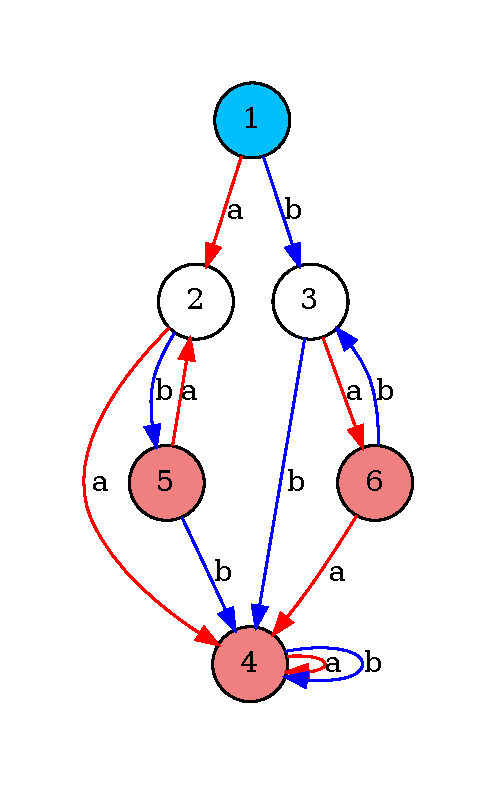
\includegraphics[width=0.5\textwidth]{images/sgpviz-2.pdf}
\end{frame}

\begin{frame}
    \begin{exampleblock}{Advantages}
        \begin{itemize}
            \item Uses graphviz standard
            \item Outputs PDFs
        \end{itemize}
    \end{exampleblock}
    \pause
    \begin{alertblock}{Challenges}
        \begin{itemize}
            \item Needs additional installation of graphviz on system
        \end{itemize}
    \end{alertblock}
\end{frame}

\subsection{Automata}
\begin{frame}{Automata (by Manuel Delgado, Steve Linton and José João Morais)}
    \begin{exampleblock}{Automata visualisation}
        \begin{itemize}
            \item Using graphviz
        \end{itemize}
    \end{exampleblock}
    \medskip
    \pause
    \centering
    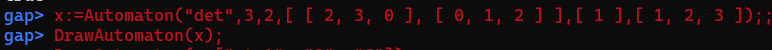
\includegraphics[width=1\textwidth]{images/automata-1.png}
\end{frame}

\begin{frame}
    \centering
    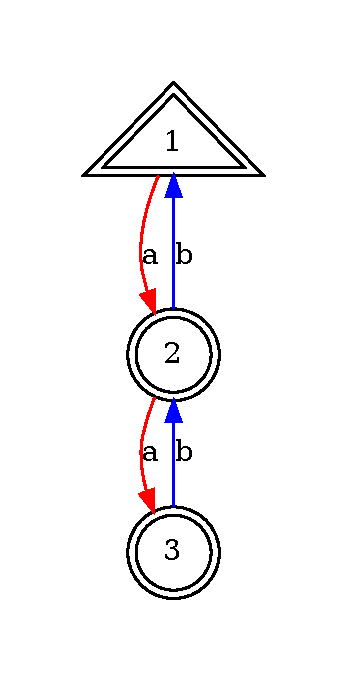
\includegraphics[width=0.4\textwidth]{images/automata-1.pdf}
\end{frame}

\begin{frame}
    \centering
    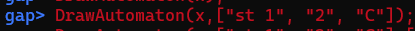
\includegraphics[width=0.7\textwidth]{images/automata-2.png}
    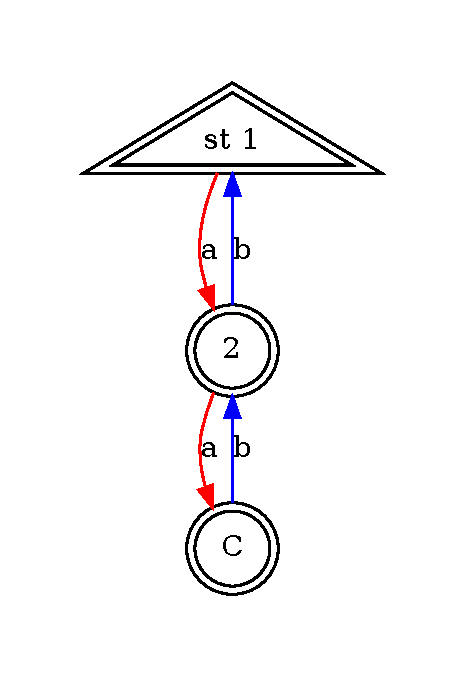
\includegraphics[width=0.5\textwidth]{images/automata-2.pdf}
\end{frame}

\begin{frame}
    \centering
    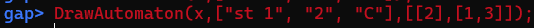
\includegraphics[width=0.7\textwidth]{images/automata-3.png}
    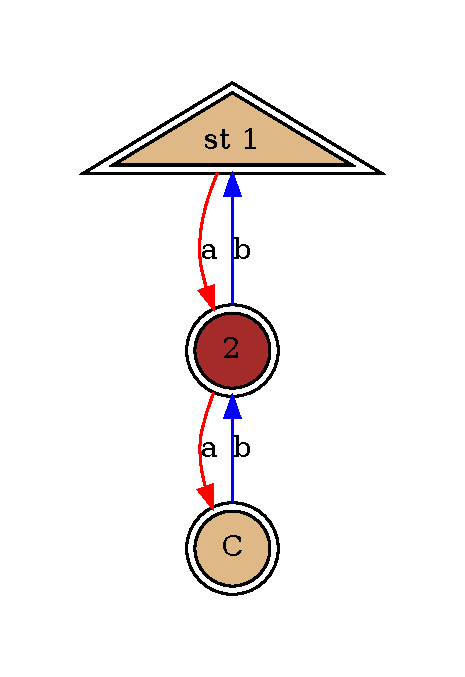
\includegraphics[width=0.5\textwidth]{images/automata-3.pdf}
\end{frame}

\begin{frame}
    \begin{exampleblock}{Advantages}
        \begin{itemize}
            \item Uses graphviz standard
            \item Outputs PDFs
        \end{itemize}
    \end{exampleblock}
    \pause
    \begin{alertblock}{Challenges}
        \begin{itemize}
            \item Needs additional installation of graphviz on system
        \end{itemize}
    \end{alertblock}
\end{frame}

\subsection{Digraphs}
\begin{frame}{graphviz (by James D. Mitchell and Matthew Pancer)}
    \begin{exampleblock}{Digraphs visualisation}
        \begin{itemize}
            \item (soon) extension to the Digraphs package
            \item Also uses graphviz standard
        \end{itemize}
    \end{exampleblock}
    \medskip
    \pause
    \centering
    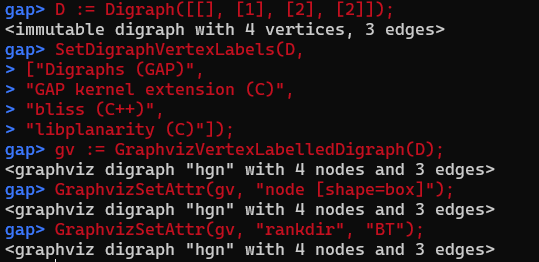
\includegraphics[width=0.8\textwidth]{images/digraphs-1.png}
\end{frame}

\begin{frame}
    \centering
    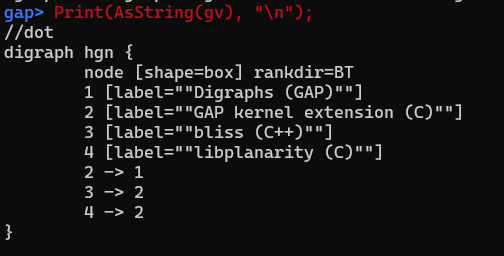
\includegraphics[width=0.6\textwidth]{images/digraphs-2.png}
    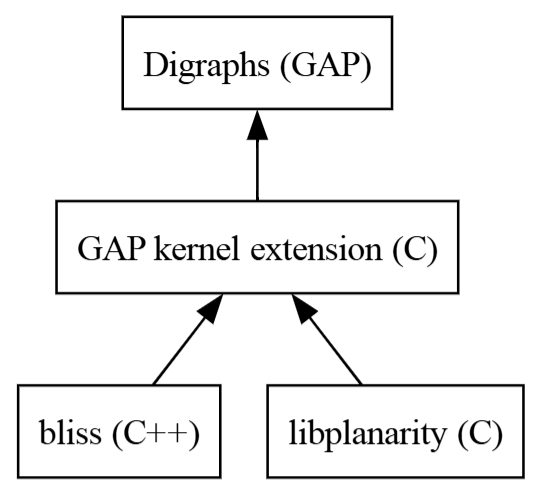
\includegraphics[width=0.39\textwidth]{images/digraphs-3.png}
\end{frame}

\begin{frame}
    \begin{exampleblock}{Advantages}
        \begin{itemize}
            \item Uses graphviz standard
            \item Is a package extension
            \item Highly customisable
            \item Visualisations can be iterated
        \end{itemize}
    \end{exampleblock}
    \pause
    \begin{alertblock}{Challenges}
        \begin{itemize}
            \item Needs GAP function for everything in graphviz standard
            \item No immediate way to show results without additional installation on system
        \end{itemize}
    \end{alertblock}
    \centering
    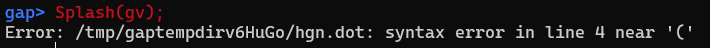
\includegraphics[width=1\textwidth]{images/digraphs-4.png}
\end{frame}

\subsection{IntPic}
\begin{frame}{IntPic (by Manuel Delgado)}
    \begin{exampleblock}{Visualises arrays of integers}
        Can be used to highlight different properties in large number of colours.
    \end{exampleblock}
    \medskip
    \pause
    \centering
    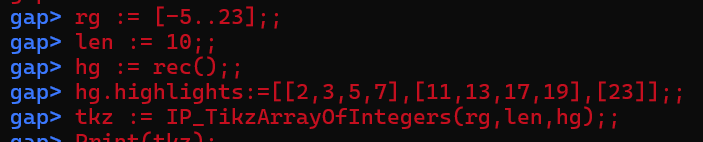
\includegraphics[width=0.9\textwidth]{images/intpic-1.png}
    
\end{frame}

\begin{frame}
    \centering
    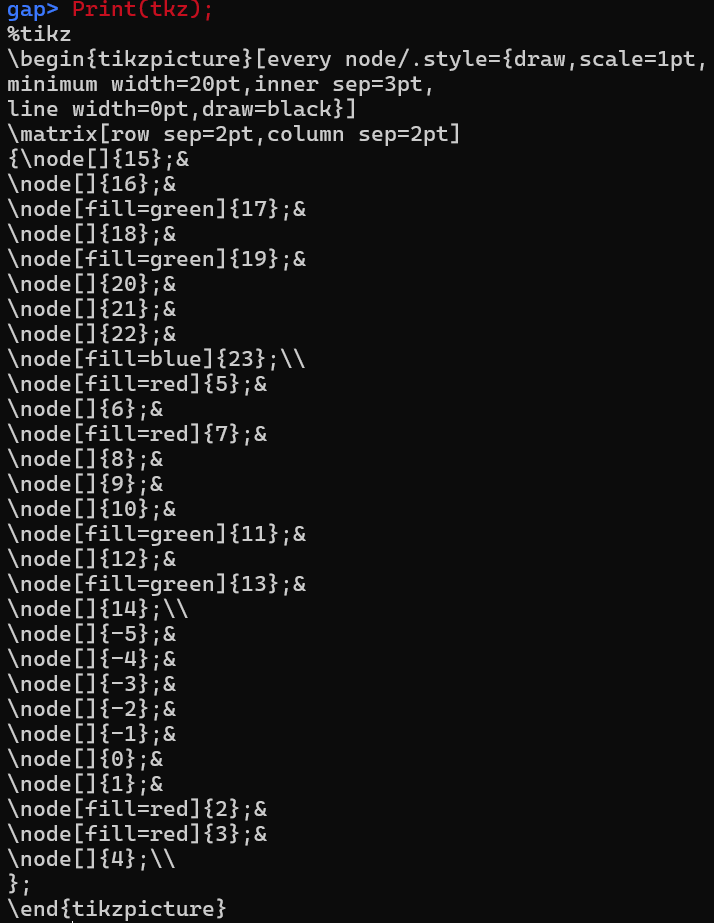
\includegraphics[width=0.4\textwidth]{images/intpic-2.png}
    %tikz
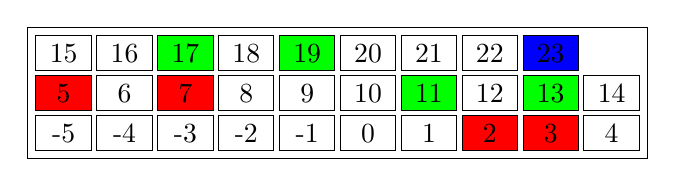
\begin{tikzpicture}[every node/.style={draw,scale=1pt,
minimum width=20pt,inner sep=3pt,
line width=0pt,draw=black}]
\matrix[row sep=2pt,column sep=2pt]
{\node[]{15};&
\node[]{16};&
\node[fill=green]{17};&
\node[]{18};&
\node[fill=green]{19};&
\node[]{20};&
\node[]{21};&
\node[]{22};&
\node[fill=blue]{23};\\
\node[fill=red]{5};&
\node[]{6};&
\node[fill=red]{7};&
\node[]{8};&
\node[]{9};&
\node[]{10};&
\node[fill=green]{11};&
\node[]{12};&
\node[fill=green]{13};&
\node[]{14};\\
\node[]{-5};&
\node[]{-4};&
\node[]{-3};&
\node[]{-2};&
\node[]{-1};&
\node[]{0};&
\node[]{1};&
\node[fill=red]{2};&
\node[fill=red]{3};&
\node[]{4};\\
};
\end{tikzpicture}
\end{frame}

\begin{frame}
    \begin{exampleblock}{Advantages}
        \begin{itemize}
            \item Uses tikz
            \item Highly customisable
        \end{itemize}
    \end{exampleblock}
    \pause
    \begin{alertblock}{Challenges}
        \begin{itemize}
            \item No immediate way to show results without compiling them
        \end{itemize}
    \end{alertblock}
    \centering
\end{frame}

\subsection{GAPic}
\begin{frame}{GAPic (by Alice C. Niemyer and many more)}
    \begin{block}{Visualising triangulated polyhedra}
        \begin{itemize}
            \item Came from the SimplicialSurfaces package
            \item Expanded functionality like general polyhedra
            \item Has SimplicialSurfaces package as extension
        \end{itemize}
    \end{block}
\end{frame}

\begin{frame}
    \centering
    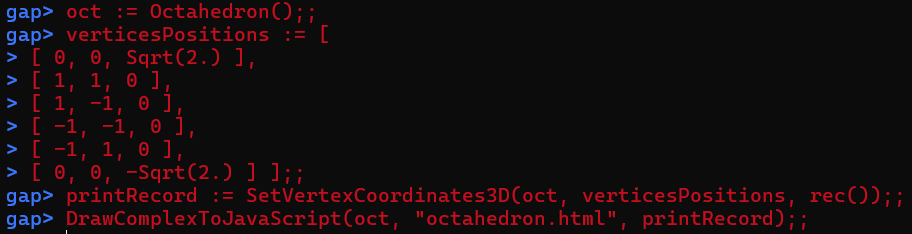
\includegraphics[width=1\textwidth]{images/gapic-1.png}
    Demonstration in browser
    \medskip
    \pause
    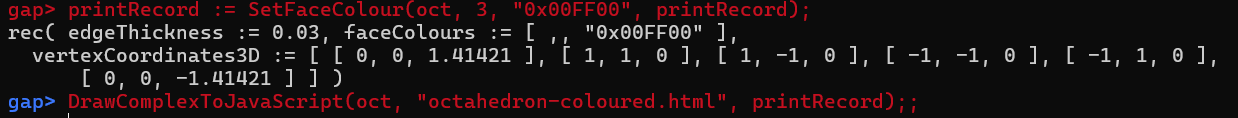
\includegraphics[width=1\textwidth]{images/gapic-2.png}
\end{frame}

\begin{frame}
    \begin{exampleblock}{Advantages}
        \begin{itemize}
            \item Results can be opened with any browser
            \item High interactivity
            \item Can use parameterised coordinates
        \end{itemize}
    \end{exampleblock}
    \pause
    \begin{alertblock}{Challenges}
        \begin{itemize}
            \item No immediate way to show results without generating them
        \end{itemize}
    \end{alertblock}
\end{frame}

\section{and}
\begin{frame}
    There are certainly more packages that include some visualisation which I did not mention.
\end{frame}

\section{The future}
\begin{frame}
    \begin{exampleblock}{Goals}
        Make visualisations in GAP...
        \begin{itemize}
            \item more visible
            \item more intuitive $\xrightarrow{}$ accessible
            \item sustainable
        \end{itemize}
    \end{exampleblock}
    \pause
    \begin{block}{Methods}
        \begin{itemize}
            \item Use of package extensions?
            \item Use of existing standards
        \end{itemize}
    \end{block}
\end{frame}

\begin{frame}{Questions and discussion}
    \begin{itemize}
        \item What are your experiences with visualisations in GAP?
        \item What do you expect from a visualisation functionality?
        \item Is there anything you want to visualise but are not able to visualise yet?
    \end{itemize}
\end{frame}

\end{document}
